%%%%%%%%%%%%%%%%%%%%%%%%%%%%%%%%%%%%%%%%%%%%%%%%%%%%%%%%%%%%%%%%%
\documentclass[hyperref={pdfpagelabels=false},compress,table]{beamer} % 在Mac下无法编译
% \documentclass[compress,table]{beamer} % 在Mac下使用
% package for font
\usepackage{fontspec}
\defaultfontfeatures{Mapping=tex-text}  %%如果没有它,会有一些 tex 特殊字符无法正常使用,比如连字符。
\usepackage{xunicode,xltxtra}
\usepackage[BoldFont,SlantFont,CJKnumber,CJKchecksingle]{xeCJK}  % \CJKnumber{12345}: 一万二千三百四十五
\usepackage{CJKfntef}  %%实现对汉字加点、下划线等。
\usepackage{pifont}  % \ding{}
% package for math
\usepackage{amsfonts}

% package for graphics
\usepackage[americaninductors,europeanresistors]{circuitikz}
\usepackage{tikz}
\usetikzlibrary{plotmarks}  % placements=positioning
\usepackage{graphicx}  % \includegraphics[]{}
\usepackage{subfigure}  %%图形或表格并排排列
% package for table
\usepackage{colortbl,dcolumn}  %% 彩色表格
\usepackage{multirow}
\usepackage{multicol}
\usepackage{booktabs}
% package for code
\usepackage{fancyvrb}
\usepackage{listings}

% \usepackage{animate}
% \usepackage{movie15}

%%%%%
% setting for beamer
\usetheme{default} % Madrid(常用), Copenhagen, AnnArbor, boxes(白色), Frankfurt,Berkeley,default
 \useoutertheme[subsection=true]{miniframes} % 使用Berkeley时注释本行
\usecolortheme{sidebartab}
\usefonttheme{serif}  %%英文使用衬线字体
% \setbeamertemplate{background canvas}[vertical
% shading][bottom=white,top=structure.fg!7] %%背景色,上25%的蓝,过渡到下白。
\setbeamertemplate{theorems}[numbered]
\setbeamertemplate{navigation symbols}{}  %% 去掉页面下方默认的导航条
\setbeamercovered{transparent}  %设置 beamer 覆盖效果

% 设置标题title背景色
% \setbeamercolor{title}{fg=black, bg=lightgray!60!white}
\setbeamercolor{title}{fg=white, bg=black!90!white}

% 设置每页小LOGO
\pgfdeclareimage[width=1cm]{ouc}{figures/static/ouc.pdf}
\logo{\pgfuseimage{ouc}{\vspace{-20pt}}}

% setting for font
%%\setCJKmainfont{Adobe Kaiti Std}
\setCJKmainfont{SimSun} 
%% \setCJKmainfont{FangSong_GB2312} 
%% \setmainfont{Apple Garamond}  %%苹果字体没有SmallCaps
\setmainfont{Times New Roman}
%FUNNY%\setCJKmainfont{DFPShaoNvW5-GB}  %%华康少女文字W5(P)
%FUNNY%\setCJKmainfont{FZJingLeiS-R-GB}  %%方正静蕾体
%FUNNY%\setmainfont{Purisa}
%\setsansfont[Mapping=tex-text]{Adobe Song Std}
     %如果装了Adobe Acrobat,可在font.conf中配置Adobe字体的路径以使用其中文字体。
     %也可直接使用系统中的中文字体如SimSun、SimHei、微软雅黑等。
     %原来beamer用的字体是sans family;注意Mapping的大小写,不能写错。
     %设置字体时也可以直接用字体名,以下三种方式等同:
     %\setromanfont[BoldFont={黑体}]{宋体}
     %\setromanfont[BoldFont={SimHei}]{SimSun}
     %\setromanfont[BoldFont={"[simhei.ttf]"}]{"[simsun.ttc]"}
% setting for graphics
\graphicspath{{figures/}}  %%图片路径
\renewcommand\figurename{图}

% setting for pdf
\hypersetup{% pdfpagemode=FullScreen,%
            pdfauthor={Xiaodong Wang},%
            pdftitle={Title},%
            CJKbookmarks=true,%
            bookmarksnumbered=true,%
            bookmarksopen=false,%
            plainpages=false,%
            colorlinks=true,%
            citecolor=green,%
            filecolor=magenta,%
            linkcolor=blue,%red(default)
            urlcolor=cyan}

% setting for fontspec
\XeTeXlinebreaklocale "zh"  %%表示用中文的断行
\XeTeXlinebreakskip = 0pt plus 1pt minus 0.1pt  %%多一点调整的空间
%%%%%

% 设置文字版式为两端对齐
\renewcommand{\raggedright}{\leftskip=0pt \rightskip=0pt plus 0cm}
\raggedright 

% font setting by xeCJK
\setCJKfamilyfont{NSimSun}{NSimSun}
\newcommand{\song}{\CJKfamily{NSimSun}}
%%%\setCJKfamilyfont{AdobeSongStd}{Adobe Song Std}
%%%\newcommand{\AdobeSong}{\CJKfamily{AdobeSongStd}}
\setCJKfamilyfont{FangSong}{FangSong_GB2312}
\newcommand{\fang}{\CJKfamily{FangSong}}
%%%\setCJKfamilyfont{AdobeFangsongStd}{Adobe Fangsong Std}
%%%\newcommand{\AdobeFang}{\CJKfamily{AdobeFangsongStd}}
\setCJKfamilyfont{SimHei}{SimHei}
\newcommand{\hei}{\CJKfamily{SimHei}}
%%%\setCJKfamilyfont{AdobeHeitiStd}{Adobe Heiti Std}
%%%\newcommand{\AdobeHei}{\CJKfamily{AdobeHeitiStd}}
\setCJKfamilyfont{KaiTi}{KaiTi}
\newcommand{\kai}{\CJKfamily{KaiTi}}
%%%\setCJKfamilyfont{AdobeKaitiStd}{Adobe Kaiti Std}
\newcommand{\AdobeKai}{\CJKfamily{AdobeKaitiStd}}
\setCJKfamilyfont{LiSu}{LiSu}
\newcommand{\li}{\CJKfamily{LiSu}}
\setCJKfamilyfont{YouYuan}{YouYuan}
\newcommand{\you}{\CJKfamily{YouYuan}}
\setCJKfamilyfont{FZJingLei}{FZJingLeiS-R-GB}
\newcommand{\jinglei}{\CJKfamily{FZJingLei}}
\setCJKfamilyfont{MSYH}{Microsoft YaHei}
\newcommand{\msyh}{\CJKfamily{MSYH}}

% 自定义颜色
\def\Red{\color{red}}
\def\Green{\color{green}}
\def\Blue{\color{blue}}
\def\Mage{\color{magenta}}
\def\Cyan{\color{cyan}}
\def\Brown{\color{brown}}
\def\White{\color{white}}
\def\Black{\color{black}}

\lstnewenvironment{javaCode}[1][]{% for Java
  \lstset{
    basicstyle=\tiny\ttfamily,%
    columns=flexible,%
    framexleftmargin=.7mm, %
    frame=shadowbox,%
    rulesepcolor=\color{cyan},%
    % frame=single,%
    backgroundcolor=\color{white},%
    xleftmargin=2\fboxsep,%
    xrightmargin=2\fboxsep,%
    %numbers=left,numberstyle=\tiny,%
    numberblanklines=false,numbersep=7pt,%
    language=Java, %
    }\lstset{#1}}{}

\lstnewenvironment{xmlCode}[1][]{% for Java
  \lstset{
    basicstyle=\tiny\ttfamily,%
    columns=flexible,%
    framexleftmargin=.7mm, %
    frame=shadowbox,%
    rulesepcolor=\color{cyan},%
    % frame=single,%
    backgroundcolor=\color{white},%
    xleftmargin=2\fboxsep,%
    xrightmargin=2\fboxsep,%
    %numbers=left,numberstyle=\tiny,%
    numberblanklines=false,numbersep=7pt,%
    language=html, %
    }\lstset{#1}}{}

\lstnewenvironment{shCode}[1][]{% for Java
  \lstset{
    basicstyle=\scriptsize\ttfamily,%
    columns=flexible,%
    framexleftmargin=.7mm, %
    frame=shadowbox,%
    rulesepcolor=\color{brown},%
    % frame=single,%
    backgroundcolor=\color{white},%
    xleftmargin=4\fboxsep,%
    xrightmargin=4\fboxsep,%
    numbers=left,numberstyle=\tiny,%
    numberblanklines=false,numbersep=7pt,%
    language=sh, %
    }\lstset{#1}}{}

\newcommand\ask[1]{\vskip 4bp \tikz \node[rectangle,rounded corners,minimum size=6mm,
  fill=white,]{\Cyan \includegraphics[height=1.5cm]{question} \Large \msyh #1};}

\newcommand\wxd[1]{\vskip 4bp \tikz \node[rectangle,minimum size=6mm,
  fill=blue!60!white,]{\White \ding{118} \msyh #1};}

\newcommand\xyy[1]{\vskip 2bp \tikz \node[rectangle,minimum size=3mm,
  fill=black!80!white,]{\White \msyh\scriptsize #1};}

\newcommand\cxf[1]{\vskip 4bp \tikz \node[rectangle,rounded corners,minimum size=6mm,
  fill=orange!60!white,]{\White \ding{42} \msyh #1};}

\newcommand\samp[1]{\vskip 2bp \tikz \node[rectangle,minimum size=3mm,
  fill=white!100!white,]{\Mage\msyh \small CODE \ding{231} \Black #1};\vskip -8bp}

\newcommand\zhyfly[1]{\tikz \node[rectangle,rounded corners,minimum size=6mm,ball
  color=red!25!blue,text=white,]{#1};}

\newcommand\pno[1]{\tikz \node[rectangle,rounded corners,minimum size=1mm,
  fill=yellow!50!black,text=white,]{\msyh\scriptsize P. #1};}

\setbeamerfont{frametitle}{series=\msyh} % 修改Beamer标题字体

\makeatletter
\newcommand{\Extend}[5]{\ext@arrow 0099{\arrowfill@#1#2#3}{#4}{#5}}
\makeatother

%%%%%%%%%%%%%%%%%%%%%%%%%%%%%%%%%%%%%%%%%%%%%%%%%%%%%%%%%%%%%%%%% 
% \titlepage
\title[KevinW@OUC]{\hei {\Large 基于Java EE的企业应用系统设计\\Spring MVC}}
\author[王晓东]{王晓东\\
  \href{mailto:wangxiaodong@ouc.edu.cn}{\footnotesize wangxiaodong@ouc.edu.cn}}
\institute[中国海洋大学]{\small 中国海洋大学}
\date{\today}
\titlegraphic{\vspace{-6em}
\includegraphics[height=6cm]{static/ouc.pdf}\vspace{-6em}}

%%%%% 
\begin{document}
%% Delete this, if you do not want the table of contents to pop up at
%% the beginning of each subsection:
\AtBeginSection[]{                              % 在每个Section前都会加入的Frame
  \frame<handout:0>{
    \frametitle{\textbf{\hei 接下来…}}
    \tableofcontents[currentsection]
  }
}  %

\AtBeginSubsection[]                            % 在每个子段落之前
{
  \frame<handout:0>                             % handout:0 表示只在手稿中出现
  {
    \frametitle{\textit{\hei 接下来…}}\small
    \tableofcontents[current,currentsubsection] % 显示在目录中加亮的当前章节
  }
}
 \frame{\titlepage}

%%%%%%%%%%%%%%%%%%%%%%%%%%%%%%%%%%%%%%%%%%%%%%%%
\begin{frame}
\frametitle{References}
\begin{enumerate}
\item Spring MVC: A Tutorial (Second Edition) (ISBN 9781771970310)
\end{enumerate}  
\end{frame}

% \begin{frame}
% \frametitle{本章学习目标}
% \begin{enumerate}
% \item 
% \end{enumerate}  
% \end{frame}

\section*{大纲}
\frame{\frametitle{大纲} \tableofcontents }

%%%%%%%%%%%%%%%%%%%%%%%%%%%%%%%%%%%%%%%%%%%%%%%%%%
\section{转换器和格式化(Converter and Formatter)}

\begin{frame}[fragile]
  \frametitle{转换器和格式化(Converter and Formatter)}

  \begin{itemize}
  \item Spring MVC框架具备数据自动绑定能力,但其数据绑定并非没有任何限
    制,在如何正确绑定数据方面是杂乱无章的。
  \item {\Red\kai 例如, Spring总是试图用默认的语言区域将日期输入绑定
      到java.util.Date}。
  \item {\hei\Blue 假如想让Spring使用不同的日期样式,就需要使
      用Converter或者Formatter。}
  \end{itemize}

  \wxd{{Converter and Formatter}}

  两者均可用于将一种对象类型转换成另一种对象类型。Converter是通用组件,
  可以在应用程序的任意层中使用,Formatter则是专门为Web层设计。

\end{frame}

\begin{frame}[fragile]
  \frametitle{Converter}
  
  Spring的Converter将一种类型转换成另一种类型的一个对象。

  {\kai 例如,用户输入的日期可能有许多种形式,如May 31,
    2017、5/31/2017和2017-05-31。默认情况下,Spring会期待用户输入的日期
    样式与当前语言区域的日期样式相同。例如,对于美国的用户而言,就是
    月/日/年格式。}

  如果希望Spring在将输入的日期字符串绑定到Date时使用不同的日期样式,则
  需要编写一个Converter,才能将字符串转换成日期。
  
\end{frame}

\begin{frame}[fragile]
  \frametitle{Converter}

  为了创建Converter,须编写实
  现\xyy{org.springframework.core.convert.converter.Converter}接口的类。
  
  \wxd{接口声明和方法}
  
  \begin{javaCode}
    public interface Converter<S, T> {
      T convert(S source);
    }
  \end{javaCode}

  S表示源类型,T表示目标类型。例如,为了创建一个可以将Long转换
  成Date的Converter,声明Converter类并实现convert方法,如下:

  \begin{javaCode}
    public class MyConverter implements Converter<Long, Date> {
      Date convert(Long source) {
        // implement the method.
      }
    }
  \end{javaCode}

\end{frame}

\begin{frame}[fragile]
  \frametitle{Converter Sample 01}

  \xyy{Converter: StringToDateConverter}
  
  \begin{javaCode}
  package converter;
  import java.text.ParseException;
  import java.text.SimpleDateFormat;
  import java.util.Date;
  import org.springframework.core.convert.converter.Converter;

  public class StringToDateConverter implements Converter<String, Date> {
    private String datePattern;

    public StringToDateConverter(String datePattern) {
      this.datePattern = datePattern;
      System.out.println("instantiating... converter with pattern:*" + datePattern);
    }

    @Override
    public Date convert(String s) {
      try {
        SimpleDateFormat dateFormat = new SimpleDateFormat(datePattern);
        dateFormat.setLenient(false);
        return dateFormat.parse(s);
      } catch (ParseException e) {
        // the error message will be displayed when using <form:errors>
        throw new IllegalArgumentException(
        "invalid date format. Please use this pattern\"" + datePattern + "\"");
      }
    }
  }
  \end{javaCode}
\end{frame}

\begin{frame}[fragile]
  \frametitle{Converter Sample 02}

  \wxd{Converter配置}

  为了使用SpringMVC应用程序中定制的Converter,需要在SpringMVC配置文件中
  编写一个conversionService bean。Bean的类名称必须
  为\xyy{org.springfamework.context.support.ConversionServiceFactoryBean},并
  包含一个converters属性,它将列出要在应用程序中使用的所有定
  制Converter。

  \xyy{StringToDateConverter配置}

  \begin{xmlCode}
    <bean id="conversionService"
      class="org.springframework.context.support.ConversionServiceFactoryBean">
      <property name="converters">
        <list>
          <bean class="converter.StringToDateConverter">
            <constructor-arg type="java.lang.String" value="MM-dd-yyyy" />
          </bean>
        </list>
      </property>
    </bean>
  \end{xmlCode}

\end{frame}

\begin{frame}[fragile]
  \frametitle{Converter Sample 02 - 续}

  然后,要给annotation-driven元素的conversion-service属性赋bean名称

  \begin{xmlCode}
    <mvc:annotation-driven conversion-service="conversionService" />
  \end{xmlCode}

\end{frame}

\begin{frame}[fragile]
  \frametitle{Converter Sample 03}

  \wxd{使用StringToDateConverter的范例应用程序}

  \xyy{Domain: Employee.java}

  \begin{javaCode}
  package domain;
  import java.io.Serializable;
  import java.util.Date;
  
  public class Employee implements Serializable {
    private static final long serialVersionUID = -908L;
    private long id;
    private String firstName;
    private String lastName;
    private Date birthDate;
    private int salaryLevel;

    // getters and setters ...
  }
  \end{javaCode}
\end{frame}

\begin{frame}[fragile]
  \frametitle{Converter Sample 03 - 续}

  \begin{javaCode}
  package controller;
  import org.springframework.ui.Model;
  import org.springframework.validation.BindingResult;
  import org.springframework.validation.FieldError;
  import org.springframework.web.bind.annotation.ModelAttribute;
  import org.springframework.web.bind.annotation.RequestMapping;
  ...
  import domain.Employee;

  @Controller
  public class EmployeeController {
    @RequestMapping(value = "input-employee")
    public String inputEmployee(Model model) {
      model.addAttribute(new Employee)
      return "EmployeeForm";
    }
    
    @RequestMapping(value = "save-employee")
    public String saveEmployee(@ModelAttribute Employee employee,
    BindingResult bindingResult, Model model) {
      if (bindingResult.hasErrors()) {
        FieldError fieldError = bindingResult.getFieldError();
        logger.info("Code:" + fieldError.getCode() + ", field:" + fieldError.getField());
        return "EmployeeForm";
        // save employee here
        model.addAttribute("employee", employee);
        return "EmployeeDetails";
      }
    }
  }
  \end{javaCode}
\end{frame}

\begin{frame}[fragile]
  \frametitle{Converter Sample 03 - 续}

  inputEmployee方法返回\xyy{EmployeeForm.jsp}页面。saveEmployee方法取出
  一个在提交Employee表单时创建的Employee对象。有
  了StringToDateConverter,就不需要在controller类中将字符串转换成日期
  了。

  saveEmployee方法的BindingResult参数中放置了Spring的所有绑定错误。该方
  法利用BindingResult记录所有绑定错误。绑定错误也可以利用errors标签显示
  在一个表单中,如

  \xyy{EmployeeForm.jsp中error标签}
  
  \begin{xmlCode}
  <p>
    <form:errors path="birthDate" cssClass="error" />
  </p>
  \end{xmlCode}

\end{frame}


\begin{frame}[fragile]
  \frametitle{Formatter}
  \begin{itemize}
  \item Formatter也是将一种类型转换成另一种类型。
  \item Formatter的源类型必须是一个String。Formatter更适合Web层,而Converter则可以用在任意层中。
  \item 为了转换Spring MVC应用程序表单中的用户输入,始终应该选择Formatter,而不是Converter。
  \end{itemize}

\end{frame}


\begin{frame}[fragile]
  \frametitle{Formatter}
  为了创建Formatter,要编写实现\xyy{org.springframework.format.Formatter}接口的类。

  \wxd{接口声明和方法}
  \begin{javaCode}
    public interface Formatter<T> {
      T parse(String text, java.util.Locale locale);
      String print(T object, java.util.Locale locale);
\end{javaCode}

T表示输入字符串要转换的目标类型,该接口有parse和print两个方法,所有实现都必须覆盖。

\begin{itemize}\kai
\item parse方法利用指定的Locale将一个String解析成目标类型。
\item print方法与之相反,它是返回目标对象的字符串表示法。
\end{itemize}

\end{frame}

\begin{frame}[fragile]
  \frametitle{Formatter Sample 01}

  \xyy{Formatter: DateFormatter.java}
  \begin{javaCode}
  package formatter;
  import java.util.Locale;
  ...
  import org.springframework.format.Formatter;

  public class DateFormatter implements Formatter<Date> {
    private String datePattern;
    private SimpleDateFormat dateFormat;
    public DateFormatter(String datePattern) {
      this.datePattern = datePattern;
      dateFormat = new SimpleDateFormat(datePattern);
      dateFormat.setLenient(false);
    }
    @Override
    public String print(Date date, Locale locale) {
      return dateFormat.format(date);
    }
    @Override
    public Date parse(String s, Locale locale) {
      try {
        return dateFormat.parse(s);
      } catch (ParseException e) {
        // the error message will be displayed when using <form:errors>
        throw new IllegalArgumentException(
        "invalid date format. Please use this pattern\" " + datePattern + " \"");
      }
    }
  }
  \end{javaCode}
  
\end{frame}

\begin{frame}[fragile]
  \frametitle{Formatter Sample 02}

  \xyy{Formatter配置}

  \begin{itemize}\kai
  \item bean
  \item context:component-scan
  \end{itemize}
  
  \begin{xmlCode}
    <bean id="conversionService"
      class="org.springframework.format.support.FormattingConversionServiceFactoryBean">
      <property name="formatters">
        <set>
          <bean class="formatter.DateFormatter">
            <constructor-arg type="java.lang.String" value="MM-dd-yyyy" />
          </bean>
        </set>
      </property>
    </bean>

    <context:component-scan base-package="formatter" />
  \end{xmlCode}

  \cxf{用Rgistrar注册Formatter}

  也可以用Registrar注册Formatter,自行搜索学习。
\end{frame}

\section{验证器}

\begin{frame}[fragile]
  \frametitle{验证器}

  输入验证是Spring处理的最重要Web开发任务之一。在Spring MVC中,可以利用Spring 自带的验证框验证用户输入。

  \begin{itemize}
  \item Converter和Formatter作用于field级。
  \item 验证器(Validator)则作用于object级,它决定某一个对象中的所有field是否均是有效的,以及是否遵循某些规则。
  \end{itemize}

\end{frame}


\begin{frame}[fragile]
  \frametitle{验证器}

  如果一个应用程序中既使用了Formatter,又有Validator,则其事件执行顺序是:
  
  \begin{enumerate}
  \item 调用Controller期间,将会有一个或者多个Formatter,试图将输入字符串转换成domain对象中的field值。
  \item 一旦格式化成功,验证器就会介入。\\
    \pause{\kai\Red 例如, Order对象可能会有一个shippingDate属性(其类
      型为Date),其值绝对不可能早于今天的日期。当调
      用OrderController时,DateFormatter会将字符串转化成Date类型,并将
      它赋给Order对象的shippingDate属性。如果转换失败,用户就会被转回到
      前一个表单。如果转换成功,则会调用验证器,查看shippingDate是否早
      于今天的日期。}
  \end{enumerate}
\end{frame}

\begin{frame}[fragile]
  \frametitle{验证器}

  为了创建Spring验证器, 要实
  现\xyy{org.springfamework.validation.Validator}接口,覆盖其
  中supports和validate两个方法。

  \wxd{Validator接口}
  
  \begin{javaCode}
    package org.springframework.validation;
    
    public interface Validator {
      boolean supports (Class<?> clazz);
      void validate (Object target, Errors errors);
    }
  \end{javaCode}

\end{frame}

\begin{frame}[fragile]
  \frametitle{验证器}
  
  \begin{itemize}
  \item 如果验证器可以处理指定的Class,supports方法将返回true。
  \item validate方法会验证目标对象, 并将验证错误填入Errors对象。
  \end{itemize}

  \xyy{Error对象}
    
  Errors对象是org.springframework.validation.Errors接口的一个实
  例。Errors对象中包含了一系列FieldError和ObjectError对象。
    
  \begin{itemize}
  \item FieldError表示与被验证对象中的某个属性相关的一个错误。例如,
    如果产品的price属性必须为负数,并且Product对象被验证为负数,那么
    就需要创建一个FieldError。
  \item 编写验证器时,不需要直接创建Error对象。给Errors对象添加错误的
    最容易的方法是在Errors对象上调用一个reject或者rejectValue方法。
  \end{itemize}
  
\end{frame}

\begin{frame}[fragile]
  \frametitle{验证器}

  \wxd{reject和rejectValue的部分方法重载}
  \begin{javaCode}
    void reject(String errorCode)
  \end{javaCode}
  \begin{javaCode}
    void reject(String errorCode, String defaultMessage)
  \end{javaCode}
  \begin{javaCode}
    void rejectValue(String field, String errorCode)
  \end{javaCode}
  \begin{javaCode}
    void rejectValue(String field, String errorCode, String defaultMessage)
  \end{javaCode}

  {\kai\Red Errors对象中的错误消息,可以利用表单标签库的Errors标签显示在HTML页面中。}
\end{frame}

\begin{frame}[fragile]
  \frametitle{ValidationUtils类}

  \xyy{org.springframework.validation.ValidationUtils}类是一个工具, 有助于编写Spring验证器。

  \xyy{OLD VERSION}
  \begin{javaCode}
    if (firstName == null || firstName.trim().isEmpty()) {
      errors.rejectValue("price");
    }
  \end{javaCode}
  
  \xyy{ValidationUtils VERSION} {\scriptsize\kai 使用rejectIfEmpty或者rejectIfEmptyOrWhitespace方法}
  \begin{javaCode}
    ValidationUtils.rejectIfEmpty("price");
  \end{javaCode}
  
  \begin{javaCode}
    ValidationUtils.rejectIfEmptyOrWhitespace("price");
  \end{javaCode}

\end{frame}

\begin{frame}[fragile]
  \frametitle{Spring MVC Validation示例}

  \cxf{References: springmvc-validation-01}

\end{frame}

\section{表达式语言(EL)}

\begin{frame}[fragile]
  \frametitle{表达式语言}

  \begin{itemize}
  \item JSP2.0最重要的特性之一就是表达式语言(EL),可以用它来访问应用程序数据。
  \item EL设计成可以轻松地编写免脚本的JSP页面,而不需要使用任何JSP声明、表达式等元素。
  \end{itemize}

  \wxd{EL的语法}
  
  \framebox{\tt \$\{expression\}}

  \begin{itemize}\kai\small
  \item 例如表达式x+y可以写成:{\tt \${x+y}},计算结果的类型为String。
  \item 如果在定制标签的属性值中使用EL表达式,那么该表达式的取值结果字
    符串将会强制变成该属性需要的类型:\\
    \framebox{\tt <my:tag someAttribute="\$\{expression\}" />}
  \end{itemize}

\end{frame}

\begin{frame}[fragile]
  \frametitle{表达式语言}

  \wxd{关键字}

  \begin{itemize}\bf\tt
  \item and eq gt true instanceof
  \item or ne le false empty
  \item not It ge null div mod
  \end{itemize}
\end{frame}


\begin{frame}[fragile]
  \frametitle{表达式语言}

  \wxd{[] 和 . 运算符}

  EL表达式可以返回任意类型的值。如果使用EL表达式操作带有属性的对象,则可以利用{\Red []或者.}运算符来访问属性。

  \begin{itemize}
  \item {[]}和.运算符类似;
  \item {[]}是比较规范的形式,运算符则比较快捷。
  \end{itemize}

  为了访问对象的属性,可以使用以下任意一种形式:
  
  \begin{itemize}\small\tt
  \item \$\{object["propertyName"]\}
  \item \$\{object.propertyName\}
  \end{itemize}  
\end{frame}
  
\begin{frame}[fragile]
  \frametitle{表达式语言(示例)}
  
  \xyy{访问隐式对象HTTP host的EL表达式}
  
  \begin{itemize}\small\tt
  \item \$\{header["host"]\}
  \item \$\{header.host\}
  \end{itemize}

  \xyy{访问accept-language的EL表达式\footnote{如果propertyNarne 不是有
      效的Java变量名,只能使用[]运算符,此处accept-language就不是合
      法Java变量名。}}

  {\small\tt \$\{header["accept-language"]\}}

\end{frame}

\begin{frame}[fragile]
  \frametitle{表达式语言(示例)}
  
  \xyy{访问pageContext.request.servletPath的EL表达式}

  隐式对象pageContext是表示当前JSP的PageContext对象,
  其HttpServletRequest request属性带有servletPath属性,下列几个表达式的
  结果相同:

  \begin{itemize}\small\tt\Blue
  \item \$\{pageContext["request"]["servletPath"]\}
  \item \$\{pageContext.request["servletPath"]\}
  \item \$\{pageContext.request.servletPath\}
  \item \$\{pageContext["request"].servletPath\}
  \end{itemize}

  \xyy{访问session的EL表达式}

  \begin{itemize}\small\tt
  \item \$\{pageContext.session\}
  \item \$\{pageContext.session.id\} 获得Session ID。
  \end{itemize}
  
\end{frame}


\begin{frame}[fragile]
  \frametitle{表达式语言}

  \wxd{访问JavaBean}

  \begin{itemize}\small\tt\Red
  \item \$\{beanName["propertyName"]\}
  \item \$\{beanName.propertyName\}
  \end{itemize}
\end{frame}

\begin{frame}[fragile]
  \frametitle{EL隐式对象}

  EL维护并提供访问隐式对象的能力。
  
  \begin{itemize}
  \item pageContext
  \item initPararm
  \item param
  \item paramValues
  \item header
  \item headerValues
  \item cookie
  \item applicationScope
  \item sessionScope
  \item requestScope
  \item pageScope
  \end{itemize}  

\end{frame}


\begin{frame}[fragile]
  \frametitle{EL隐式对象(示例)}

  \wxd{param}

  隐式对象param用于获取请求参数值,该对象表示一个包含所有请求参数的Map。

  \framebox{\tt \$\{param.userName\}} 获取userName参数。

  \wxd{cookie}

  隐式对象cookie可以用来获取一个cookie。这个对象表示当
  前HttpServletRequest中所有cookie的值。{\kai\Red 例如,为了获取名
    为jsessionid 的cookie 值,要使用以下表达式:}

  \framebox{\tt \$\{cookie.jsessionid.value\}}
  
  {\kai\Red 获取jsessionid cookie的路径值要使用以下表达式:}

  \framebox{\tt \$\{cookie.jsessionid.path\}}
  
\end{frame}

\begin{frame}[fragile]
  \frametitle{EL隐式对象(示例)}

  \wxd{applicationScope, sessionScope, requestScope, pageScope}
  \begin{itemize}
  \item 隐式对象applicationScope用于获取应用程序范围级变量的值,其他类似。

    {\Red\tt \$\{applicationScope.myVar\}}

  \item 有界对象
    (PageContext、ServletRequest、HttpSession或ServletContext)也可以
    通过没有范围的EL表达式获取。在这种情况下,JSP容器将按照由大到小的范
    围返回PageContext、ServletRequest、HttpSession或ServletContext中第
    一个同名的对象。

    {\Red\tt \$\{today\}}
    
  \end{itemize}

\end{frame}

\begin{frame}[fragile]
  \frametitle{EL运算符}

  请自行搜索学习EL其他运算符的使用。

  \begin{description}
  \item [算术运算符] + - * / div \% mod
  \item [逻辑运算符] \&\& and || or ! not
  \item [关系运算符] == eq != ne ...
  \item [empty运算符] {\tt \$\{empty X\}}
  \end{description}
\end{frame}

\begin{frame}[fragile]
  \frametitle{EL配置}

  \wxd{实现兔脚本的JSP页面}
  
  为了关闭JSP页面中的脚本元素,要使用jsp-property-group元素以
  及url-patern和scripting-invalid两个子元素。

  url-pattern元素定义禁用脚本要应用的URL样式。例如如何将一个应用程序中所有JSP页面的脚本都关闭:

  \begin{xmlCode}
    <jsp-config>
      <jsp-property-group>
        <url-pattern>*.jsp</url-pattern>
        <scripting-invalid>true</scripting-invalid>
      </jsp-property-group>
    </jsp-config>
  \end{xmlCode}

  {\small\kai\Red 注意:在部署描述符web.xml中只能有一个jsp-config元素。
    如果已经为禁用EL而定义了一个jsp-property-group,就必须在同一
    个jsp-config元素下,为禁用脚本而编写jsp-property-group。}

\end{frame}

\begin{frame}[fragile]
  \frametitle{JSP EL示例}

  \cxf{References: springmvc-validation-01}

  访问get-elsamples端点。

\end{frame}



\section{JSTL}

\begin{frame}[fragile]
  \frametitle{JSTL}

  {\hei JSP标准标签库(Java Server Pages Standard Tag Library, JSTL)}是一个定
  制标签库的集合,用来解决像遍历map或集合、条件测试、XML处理,甚至是数
  据库访问和数据操作等常见的问题。


  \wxd{下载JSTL}
  
  JSTL是由JSR-52专家组在JCP(www.jcp.org)上定义的,下载地址:{\bf\Red
    http://jstl.java.net}
  
  其中,JSTL API和JSTL实现这两个软件包必需下载。
  
  \begin{itemize}\kai\Blue
  \item JSTL API中javax.servlet.jsp.jstl包含了JSTL规范中定义的类型。
  \item JSTL实现中包含实现类。
  \item 这两个jar文件都必须复制到应用JSTL的每个应用程序的WEB-INF/lib目
    录下。
  \end{itemize}

\end{frame}

\begin{frame}[fragile]
  \frametitle{JSTL标签库}

  JSTL是标准标签库,通过{\hei\Red 多个标签库}来暴露其行为。
  
  \begin{figure}
    \centering
    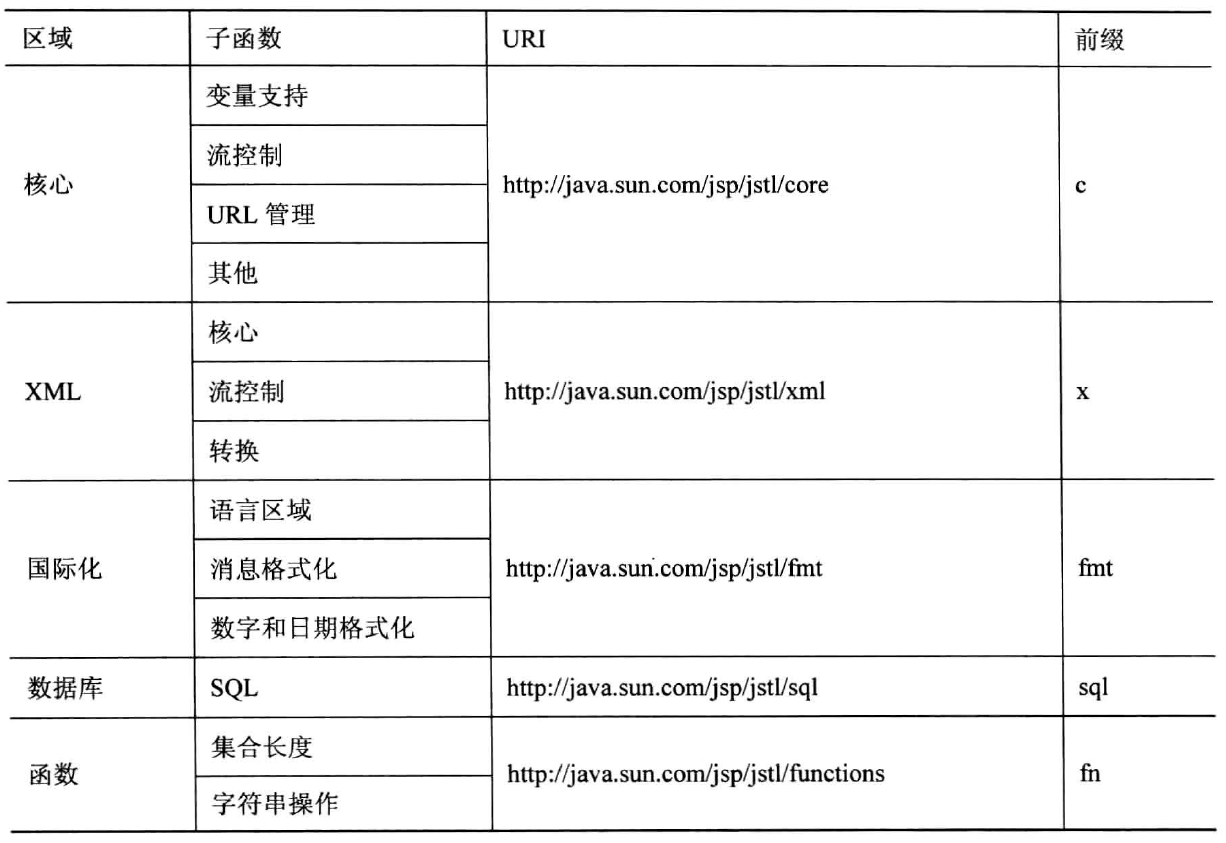
\includegraphics[width=0.9\textwidth]{jstl-taglibs.png}
  \end{figure}
\end{frame}

\begin{frame}[fragile]
  \frametitle{JSTL标签库的使用}

  \wxd{在JSP页面中使用JSTL库,必须通过以下格式使用taglib指令}

  
  \framebox{\tt\small <\%@ taglib uri="uri" prefix="prefix" \%>}

  \xyy{使用Core库}

  \framebox{\tt\scriptsize <\%@ taglib uri="http://java.sun.com/jsp/jstl/core"
    prefix="c" \%>}\footnote{前缀可以是任意的。但采用惯例能使团队的其他
    开发人员以及后续加入该项目的其他人员更容易熟悉代码。建议使用预定的
    前缀。}

\end{frame}

\begin{frame}[fragile]
  \frametitle{JSTL一般标签}

  \wxd{out标签}

  out标签在运算表达式时,是将结果输出到当前的JspWriter。

  \begin{xmlCode}
    <c: out value="value" [escapeXml=" {true|false}"][default="defaultValue"] />
  \end{xmlCode}

  \begin{xmlCode}
    <c:out value="value" [escapeXml="{true|false}"]>
      default value
    </c:out>
  \end{xmlCode}

\end{frame}

\begin{frame}[fragile]
  \frametitle{JSTL一般标签}

  \wxd{set标签}

  利用set标签,可以完成以下工作:

  \begin{itemize}
  \item 创建一个字符串和一个引用该字符串的有界变量。
  \item 创建一个引用现存有界对象的有界变量。
  \item 设置有界对象的属性。
  \end{itemize}

  用set创建的有界变量在该标签出现后的整个JSP页面中都可以使用该变量。
  
\end{frame}

\begin{frame}[fragile]
  \frametitle{JSTL一般标签}
  
  \wxd{set标签}

  第一种形式用于创建一个有界变量,并用value属性在其中定义一个要创建的字符串或者现存有界对象。

  \begin{xmlCode}
    <c:set va1ue="va1ue" var="varName"
    [scope="{page|request|session|app1ication}"] />
  \end{xmlCode}

  这里的scope属性指定了有界变量的范围。

  {\kai\Red 例如,下面的set标签创建了字符串“The wisest fool”,并将它赋给
    新创建的页面范围变量foo:}

  \begin{xmlCode}
    <c:set var="foo" value="The wisest foo1" />
  \end{xmlCode}

\end{frame}


\begin{frame}[fragile]
  \frametitle{JSTL一般标签}

  \wxd{set标签}
  
  如下的set标签则创建了一个名为job的有界变量,引用请求范围的对
  象position;out标签在运算表达式时,是将结果输出到当前的JspWriter。

  \begin{xmlCode}
    <c: set var="job" value="\${requestScope.position}" scope="page"/>    
  \end{xmlCode}

  {\kai\Red 因Emacs格式高亮原因,被迫在代码中添加了反斜线以转义字符,注意删除,以下同。}

\end{frame}


\begin{frame}[fragile]
  \frametitle{JSTL一般标签}

  \wxd{remove标签}

  remove标签用于删除有界变量。

  {\kai 有界变量引用的对象不能删除。因此,如果另一个有界对象也引用了同
    一个对象,仍然可以通过另一个有界变量访问该对象。}
  
  \begin{xmlCode}
    <c:remove var="varName" [scope="{pagelrequest lsession lapplication}"] />  
  \end{xmlCode}

  \xyy{Sample}

  下面的remove标签删除了页面范围的变量job:
  \begin{xmlCode}
    <c:remove var="job" scope="page" />
  \end{xmlCode}

\end{frame}

\begin{frame}[fragile]
  \frametitle{JSTL条件行为标签}

  {\hei JSTL中执行条件行为的有4个标签,即if、choose、when和otherwise标签。}

  \wxd{if标签}

  if标签是对某一个条件进行测试,假如结果为True,就处理它的body content。
  测试结果保存在Boolean对象中,并创建有界变量来引用这个Boolean对象。利
  用var属性和scope属性分别定义有界变量的名称和范围。

  \begin{xmlCode}
    <c:if test="testCondition" var="varName"
    [scope="{page|request|session|application}"] />
  \end{xmlCode}

  \begin{xmlCode}
    <c:if test="testCondition" [var="varName"] [scope="{page|request|session|application}"]>
      body content
    </c:if>
  \end{xmlCode}
\end{frame}

\begin{frame}[fragile]
  \frametitle{JSTL条件行为标签}
  
  \wxd{choose + when + otherwise}

  其作用与Java中的关键字switch类似。

  \begin{xmlCode}
    <c:choose>
      <c:when test="\${param.status=='full'}">
        You are a full member
      </c:when>
      <c:when test="\${param.status=='student'}">
        You are a student member
      </c:when>
      <c:otherwise>
        Please register
      </c:otherwise>
    </c:choose>
  \end{xmlCode}

\end{frame}

\begin{frame}[fragile]
  \frametitle{JSTL遍历行为标签}

  \wxd{forEach标签}

  固定次数地重复body content:
  
  \begin{xmlCode}
    <c:forEach [var="varName"] begin="begin" end="end" step="step">
      body content
    </c:forEach>
  \end{xmlCode}

  \xyy{Sample}

  \begin{xmlCode}
    <c:forEach var="x" begin="l" end="5">
      <c:out value="\${x}" />
    </c:forEach>
  \end{xmlCode}

\end{frame}

\begin{frame}[fragile]
  \frametitle{JSTL遍历行为标签}

  \wxd{forEach标签}

  遍历对象集合:
  
  \begin{xmlCode}
    <c:forEach items="collection" [var="varName"]
    [varStatus="varStatusName"] [begin="begin"] [end="end"] [step="step"] >
      body content
    </c:forEach>  
  \end{xmlCode}

  \xyy{Sample}

  \begin{xmlCode}
    <c:forEach var="phone" items="\${address.phones}">
      \${phone}" <br/>
    </c:forEach>
  \end{xmlCode}

\end{frame}

\begin{frame}[fragile]
  \frametitle{URL相关行为标签}

  \wxd{url标签}



\end{frame}


\begin{frame}[fragile]
  \frametitle{URL相关行为标签}

  \wxd{redirect标签}


\end{frame}


\begin{frame}[fragile]
  \frametitle{格式化标签和函数}

  \cxf{请自行学习,随用随学!}


\end{frame}


% \section{Spring拦截器实现用户登录验证}
% \section{Spring文件上传和下载}




% TKS %%%%%%%%%%%%%%%%%%%%%%%%%%%%%%%%%%%%%%%%%%%%
\begin{frame}
  \centering
  {\Huge \textcolor{blue}{THE END}} \\
  \vspace{5mm}
  {\Large wangxiaodong@ouc.edu.cn} \\
\end{frame}
%%%%%%%%%%%%%%%%%%%%%%%%%%%%%%%%%%%%%%%%%%%%%%%%%%
\end{document}
